\documentclass[11pt,a4paper]{article}
% Packages
\usepackage[utf8]{inputenc}
\usepackage[spanish, es-tabla]{babel}
\usepackage{caption}
\usepackage{listings}
\usepackage{adjustbox}
\usepackage{enumitem}
\usepackage{boldline}
\usepackage{amssymb, amsmath}
\usepackage[margin=1in]{geometry}
\usepackage{xcolor}
\usepackage{soul}
\usepackage{graphicx}
\graphicspath{ {../images/} }

% Meta
\title{Bitcoin}
\author{Guillermo Galindo Ortuño, Carlos Santiago Sánchez Muñoz}
\date{\today}

% Custom
\providecommand{\abs}[1]{\lvert#1\rvert}
\setlength\parindent{0pt}
\definecolor{Light}{gray}{.90}
\newcommand\ddfrac[2]{\frac{\displaystyle #1}{\displaystyle #2}}

\begin{document}
\begin{titlepage}
  \centering
  
  \vspace{10cm}
  
\includegraphics[width=0.4\textwidth]{bitcoinlogo2.jpeg}\par\vspace{1cm}
  {\scshape\large Fundamentos de Redes \par} \vspace{1cm}
  \vspace{0.4cm}
  {\large\itshape Redes P2P y Bitcoin\\}
  \vspace{0.6cm}
  {\large\itshape  Guillermo Galindo Ortuño\\Carlos Santiago Sánchez Muñoz \par} \vspace{1.00cm}

  \vfill
  % Bottom of the page
  {\large \today\par}

\end{titlepage}
\tableofcontents
\newpage

\section{Peer-to-peer (P2P)}
\subsection{Introducción}
P2P es una arquitectura para aplicaciones de computación distribuida en la que no existe la distinción usual de cliente-servidor, sino que cada nodo actua ``simultaneamente'' como cliente y como servidor (Imagen 1). Esto significa que cada ordenador puede actuar como cliente y solicitar un ``archivo'' a la red, de manera que actúen como servidores el resto de nodos que posean dicho archivo, y tras descargar este archivo, el nodo que lo solicitó pasará a actuar como servidor para futuras solicitudes de ese archivo.\\

Esta arquitectura se dio a conocer en el mundo entero con el lanzamiento en 1999 de Napster, una aplicacion destinada a compartir archivos (principalmente enfocada a archivos de música) que utilizaba una arquitectura P2P, lo que permitía que millones de usuarios se pudiesen conectar entre ellos directamente, y poder compartir cualquier archivo con velocidades de descarga bastante altas. Tras esto, esta arquitectura se hizo muy popular,y numerosas aplicaciones la han utilizado tales como \textit{Spotify, Skype, bitcoin, bitTorrent,}  etc.\\

\begin{figure}[h]
	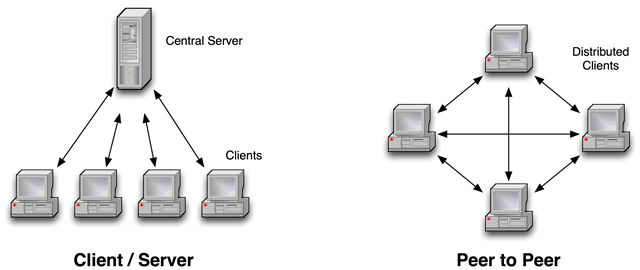
\includegraphics[width=12cm]{clientserverp2p}
	\centering		
	\caption{Cliente-Servidor vs P2P}
	\label{p3}
\end{figure}

En esta presentación trataremos sobre cuáles son las principales características de esta arquitectura, las ventajas e inconvenientes de esta, algunas de las aplicaciones mencionadas anteriormente.

\subsection{Características}
La características de esta red entre iguales son:\\

\begin{itemize}

	\item \textbf{Escalabilidad}. Estas redes ienen un alcance mundial con millones de usuarios, por eso lo deseable es que cuantos más nodos estén conectados a una red P2P, mejor sea su funcionamiento. Por tanto, cuando los nodos llegan y comparten sus propios recursos, los recursos del sistema aumentan. Sin embargo, en las arquitecturas cliente-servidor con un sistema fijo de servidores, la adición de clientes podría significar una transferencia de datos más lenta para todos los usuarios.
	
	\item \textbf{Robustez}. Las redes peer-to-peer tienen una naturaleza distribuida por lo que se incrementa la robustez en caso de haber fallos en la réplica excesiva de los datos hacia múltiples destinos.
	
	\item \textbf{Descentralización}. Estas redes por definición son descentralizadas y todos los nodos son iguales. No existen nodos con funciones especiales, y por tanto ningún nodo es imprescindible para el funcionamiento de la red. En realidad, algunas redes comúnmente llamadas P2P no cumplen esta característica, como Napster, eDonkey o BitTorrent.
	
	\item \textbf{Distribución de costes entre los usuarios}. Se comparten o donan recursos a cambio de recursos. Estos recursos pueden ser archivos, ancho de banda, ciclos de proceso, almacenamiento de disco…
	
	\item \textbf{Anonimato}. Es deseable que en estas redes quede anónimo el autor de un contenido, el editor, el lector, el servidor que lo alberga y la petición para encontrarlo, siempre que así lo necesiten los usuarios. Con frecuencia el derecho al anonimato y los derechos de autor son incompatibles, por lo que se proponen mecanismos como el DRM (Digital Rights Management) para limitar ambos.
	
	\item \textbf{Seguridad}. Es una de las características deseables de las redes P2P menos implementada. Los objetivos de un P2P serían identificar y evitar los nodos maliciosos, el contenido infectado, el espionaje de las comunicaciones entre nodos, creación de grupos seguros de nodos dentro de la red, protección de los recursos de la red... La mayor parte de los nodos aún están bajo investigación, pero los mecanismos más prometedores son: cifrado multiclave, cajas de arena, gestión de derechos de autor (la industria define qué puede hacer el usuario; por ejemplo, el usuario sólo puede descargar el archivo una vez), reputación (permitir acceso sólo a los conocidos), comunicaciones seguras, etc.
	
\end{itemize}

\subsection{Clasificación}

\begin{itemize}
	\item \textbf{Redes desestructuradas:} como su propio nombre indica, son redes en las que no se impone una estructura particular a la hora del diseño de la red, sino que los nodos están conectados de manera ``aleatoria" (Figura 2).

Las ventajas de este tipo de arquitectura son que es fácil añadir nodos, y que son redes muy resistentes a fallos ya que la caída de un nodo no afecta prácticamente al funcionamiento del sistema.

El principal inconveniente se da a la hora de buscar un dato en específico en la red, donde la falta de una estructura significa que tengas que mandar mensajes a cada uno de los nodos en busca de dicho dato, lo que provoca un riesgo alto de sobrecarga en la red.

\begin{figure}[h]
	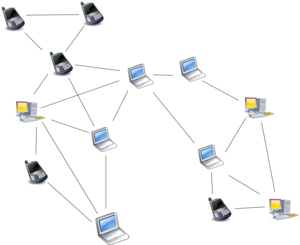
\includegraphics[width=8cm]{Unstructured.png}
	\centering		
	\caption{Desectructuradas}
	\label{p5}
\end{figure}

	\item \textbf{Redes estructuradas:} En este tipo de redes el diseño se rige por una determinada topología, asegurando así que cada nodo puede buscar de manera eficiente cualquier archivo por extraño que sea. Esto se suele implementar mediante una tabla hash distribuida, de manera que se conoce qué nodos poseen determinado archivo, así como cada nodo posee una lista de "vecinos" que cumplen una serie de criterios (Figura 3).

Esta estructura tiene como principal inconveniente que es mas propensa a sobrecargarse si se están añadiendo y eliminando nodos continuamente.

\begin{figure}[h]
	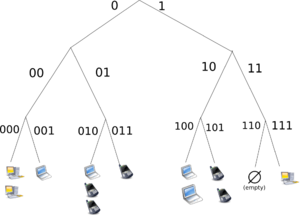
\includegraphics[width=8cm]{Structured.png}
	\centering		
	\caption{Estructuradas}
	\label{p5}
\end{figure}

	\item \textbf{Modelo híbrido:} combinan peer-to-peer y cliente/servidor. Tenemos un servidor central que ayuda a los nodos a encontrarse. Actualmente este modelo tiene un mejor rendimiento que los puros desectructurados o estructurados ya que algunas funciones como la búsqueda requieren una funcionalidad centralizada pero se aprovechan de los beneficios de la agregación descentralizada de nodos proporcionada por redes no estructuradas. Un ejemplo de este modelo sería \textit{Spotify}.

\end{itemize}

\subsection{Problemas de funcionamiento}
La mayor parte de los nodos de Internet no disponen de una dirección IP fija o accesible para otros nodos de Internet. Por ejemplo los nodos que se conectan a través de redes locales como Wifi o Ethernet, de aquellos que tienen algún tipo de cortafuegos y NAT o de los que se conectan a través de la mayor parte de los ISPs del mundo.\\

Para el correcto funcionamiento de una red P2P, hay que resolver dos problemas:

\begin{itemize}

	\item \textbf{Cómo se encuentra un nodo que ya esté conectado a la red P2P.}

La solución habitual es realizar una conexión a un servidor (o servidores) inicial con dirección bien conocida que el programa P2P tiene almacenada. Este servidor inicial se encarga de mantener una lista con las direcciones de otros nodos que están conectados a la red en ese momento. Tras esto, los clientes disponen de información suficiente para entrar en la red y pueden intercambiar información con otros nodos, ya sin intervención de los servidores iniciales.

	\item \textbf{Cómo se conectan los nodos sin dirección IP pública entre ellos.}

La solución es una conexión a través de otro nodo que funciona como proxy de la conexión. Los dos nodos se conectan al proxy y éste envía la información que llega de uno al otro. Cualquier nodo con una dirección IP pública puede ser escogido como proxy de una conexión entre dos nodos. Por ejemplo, en Skype a través de nuestro ordenador pueden pasar conversaciones de otras personas. Aquí es imprescindible la implementación de  mecanismos de seguridad para evitar que los proxies puedan llegar a entender la comunicación entre los dos nodos.

\end{itemize}

\underline{Nota:} Un \textbf{proxy} es un ordenador intermedio que se usa en la comunicación de otros dos. La información va directamente entre un ordenador y otro. Mediante un proxy, la información va primero al proxy y éste lo envía al ordenador de destino.

\section{Introducción a Bitcoin}

Como ya hemos comentado hay diversas aplicaciones que se basan en P2P como \textit{eDonkey, BitTorrent, eMule, SopCast…} Queremos centrar nuestro trabajo e investigación en una de ellas: Bitcoin.\\

Bitcoin es una criptodivisa que fue concebida en 2009, cuyo fundador es Satoshi Nakamoto, del que a parte de ser de Japón no se conoce mucho más. El término de bitcoin, a parte de usarse para referirse a la unidad monetaria, se utiliza tambien para denominar al protocolo y a la red P2P que lo sustenta. Esta se ha hecho muy popular, tanto es así que ahora mismo un bitcoin esta valorado en aproximadamente 5000\$, y tambien a raíz de ella han aparecido otras criptodivisas como Ethereum, etc.\\

Una de las características fundamentales de Bitcoin es que es completamente descentralizado, es decir, no requiere de un servidor de central o de entidades como bancos, etc que controlen el tráfico. Esto se consigue gracias a la red P2P mencionada anteriormente, y a la llamada \emph{cadena de bloques}, que es el mecanismo que utiliza la red para almacenar y controlar todas las transacciones que se realizan.

\begin{figure}[h]
	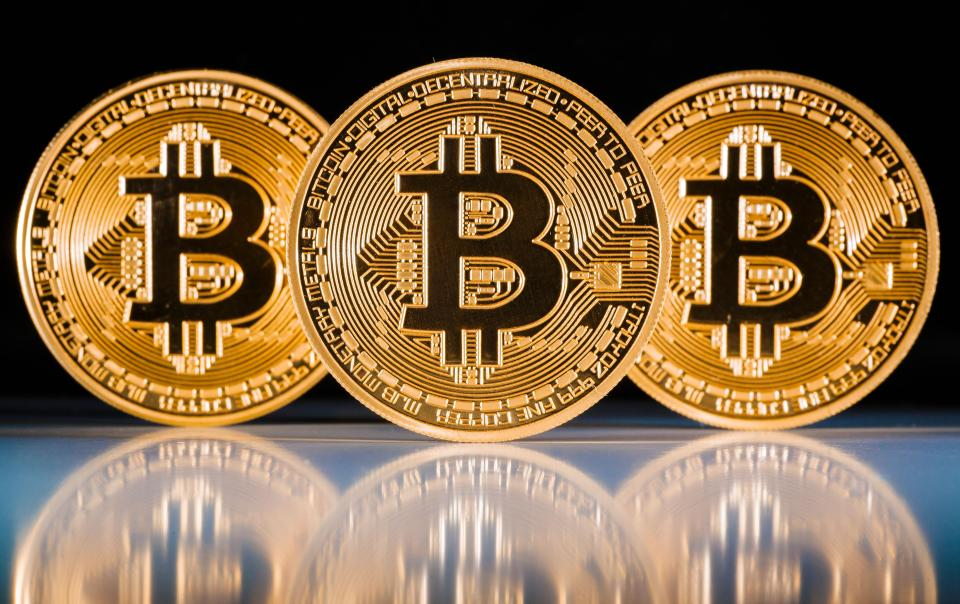
\includegraphics[width=8cm]{bitcoin.jpg}
	\centering		
	\caption{Símbolo de bitcoin}
	\label{p5}
\end{figure}

\section{La cadena de bloques}
\subsection{Estructura de bloque}
Como dijimos antes, la cadena de bloques es el sistema que utiliza Bitcoin para almacenar y controlar las transacciones de la red. Esta está formado por bloques, en los cuales se almacenan las transacciones y que están 'conectados' entre ellos, formando una estructura similar a una cadena. Cada nodo de la red almacena independientemente una cadena de bloques validados por él mismo, y cuando varios bloques tienen los mismos bloques en su cadena se dice que estan en ``consenso''. El hecho de validar bloques es a lo que usualmente se llama ``minar", y consiste a grandes rasgos en crear bloques a partes de transacciones y comprobar que son 'correctas'.\\

Cada bloque posee la siguiente estructura:

\begin{figure}[h]
	\centering
	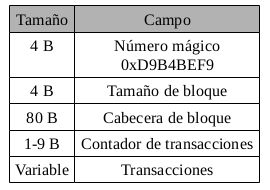
\includegraphics[width=6cm]{blockstructure.png}			
	\caption{Estructura de cada bloque}
	\label{p1}
\end{figure}

Como podemos observar, cada bloque posee, en primer lugar, un número magico que sirve para identificar el tipo de estructura utilizada(esto no es algo propio de bitcoin), el tamaño de bloque, la cabecera(de lo que hablaremos a continuación), el número de transacciones incluidas en dicho bloque y por último el conjunto de transacciones de dicho bloque. La cabecera es la parte fundamental de un bloque y posee la siguiente estructura:\\

\begin{figure}[h]
	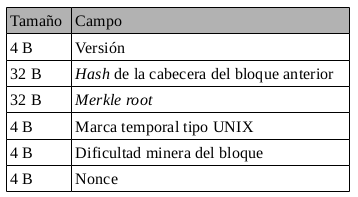
\includegraphics[width=8cm]{headerstructure.png}
	\centering		
	\caption{Estructura la cabecera de cada bloque}
	\label{p2}
\end{figure}

Aqui se muestra como en la cabecera se encuentra, la versión del protocolo utilizado, un hash de la cabecera anterior que es lo que conecta cada bloque a la cadena, el \emph{merkle root} de lo que hablaremos más adelante, una marca temporal que especiifica el momento en que ha sido añadido dicho bloque(en concreto es el tiempo que ha pasado desde 1970), un indicador de la dificultad de validar dicho bloque, y luego un conjunto de bits arbitrarios utilizados a la hora de recalcular el hash de dicho bloque.

\begin{figure}[h]
	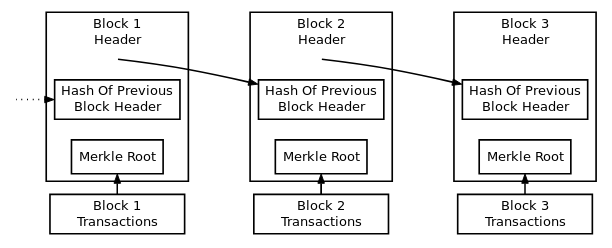
\includegraphics[width=12cm]{blockchain.png}
	\centering		
	\caption{Ejemplo simplificado de una cadena de bloques}
	\label{p3}
\end{figure}

En la figura \ref{p3} podemos ver una representación simplificada de una cadena de bloques. Es gracias a esta estructura que intentar modificar maliciosamente una transacción para obtener un beneficio ``ilegal'' es una acción prácticamente imposible de realizar ya que requeriría una capacidad computacional inmensa, debido a que tendrías que volver a validar todos los bloques que cuelguen del bloque que se desea modificar.\\

\subsection{Transacciones}

Como mencionamos anteriormente, un bloque de una o varias nuevas transacciones se almacena en la sección de datos de un bloque. Estas transacciones se almacenan encadenadas, de forma parecida a como lo hacen los bloques. Aunque de la impresion de que los satoshis van de una cartera a otra, en realidad estos van de transacción en transacción. Cada transacción gasta los satoshis recibidos anteriormente de transacciones previas. De esta manera la entrada de una transacción esta formada por partes de la salida de otras transacciones. \\

\begin{figure}[h]
	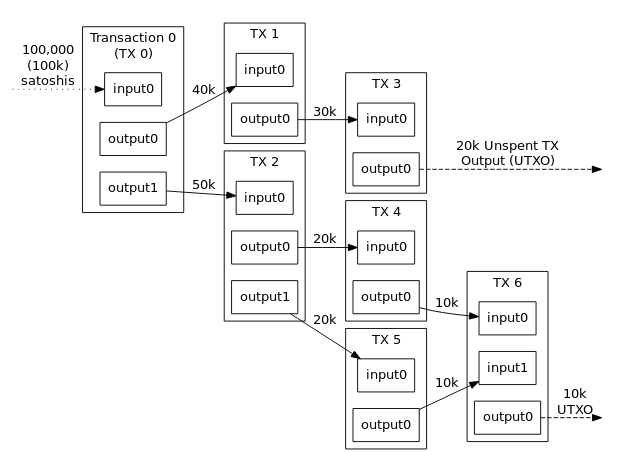
\includegraphics[width=12cm]{transactions.png}
	\centering		
	\caption{Ejemplo de la relación entre transacciones}
	\label{p4}
\end{figure}

Como podemos ver en la imagen, una transacción puede crear múltiples salidas, pero cada salida puede utilizarse una única vez como entrada de otra transacción, impidiendo así que los mismos satoshis se dupliquen 'ilegalmente'. Debido a esto, todas las salidas se pueden agrupar en 'Salidas no gastadas'(UTXOs) o en salidas gastadas. Para que un pago sea válido únicamente debe utilizar UTXOs como entradas. Para que una transacción sea válida, es necesario que el número de satoshis gastados no sea mayor que la entrada, y en caso de que la entrada sea mayor que la salida, los satoshis de diferencia son considerados como la tasa que se lleva el nodo minero por validar dichas transacciones.\\

%TODO: Buscar de donde proviene la entrada de la coinbase transaction

Tener que descargar el arbol entero cada vez que se quisiera comprobar si una transacción se encuentra en un bloque sería muy costoso, y es por eso que se utilizan los llamados 'merkle tree' y 'merkle root'. El merkle tree es un arbol que se construye aplicando hash a cada transacción, y luego a cada pareja de hashes, y así recursivamente hasta llegar a un único hash, que es a lo que llamamos merkle root, y que está almacenado en la cabecera de cada bloque. A continuación mostramos un ejemplo de como se construiría un merkle tree a partir del conjunto de transacciones ABCDE.

\begin{figure}[h]
	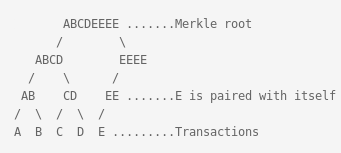
\includegraphics[width=8cm]{merkleroot.png}
	\centering		
	\caption{Ejemplo simplificado de un merkle tree}
	\label{p5}
\end{figure}

Gracias a esto, se reduce enórmemente el coste necesario para comprobar si una transacción está en un bloque o no. Por ejemplo, para comprobar en este caso si la transacción E está en el árbol, únicamente sería necesario el hash ABCD y el hash de E.\\

\subsection{Prueba de trabajo}
La cadena de bloques se mantiene gracias al trabajo de una serie de nodos anónimos en la red, por lo que Bitcoin necesita una prueba de que una cierta cantidad de trabajo ha sido invertida en la creación de un bloque, para asegurarse que nodos 'malignos' que quieran modificar un bloque ya validado tengan que realizar mas trabajo que los nodos 'buenos' que simplemente quieran añadir un nuevo bloque a la cadena.\\

El principal beneficio de la estructura de la cadena de bloques es que para modificar las transacciones de uno de los bloques de la cadena, habría que recalcular el hash de cada bloque que cuelgue de él, lo que resulta en un coste computacional prácticamente inalcanzable.\\

La prueba de trabajo que utiliza Bitcoin se aprovecha de la aparente naturaleza aleatoria de las funciones hash cryptográficas. A continuación explicaremos como funciona esta prueba: la manera de probar que has realizado un determinado trabajo para para crear un bloque es crear un hash de la cabecera de dicho bloque que sea menor que un valor en concreto. Por ejemplo, si el valor máximo alcanzable por la función hash es $2^{256}-1$, entonces produciendo un hash por debajo de $2^{254}$ probarías que has realizado cerca de 4 intentos para producir dicho hash.\\

De esta manera, nuevos bloques serán añadidos únicamente si cumplen la condición de que la difucultad para crearlos cumple con el valor esperado por el protocolo de consenso, es decir si el hash de dicho bloque está por debajo de un valor que es el que marca dicha dificultad. Cada 2016 bloques se usa la marca de tiempo que hay en cada bloque para calcular el tiempo que han tardado estos 2016 bloques en producirse, siendo el valor ideal dos semanas aproximandamente. La dificultad esperada variará con el objetivo de que los siguientes 2016 bloques se produzcan en un tiempo lo más cercano posible a dos semanas, de la siguiente manera:
\begin{itemize}
	\item Si tomó más de dos semanas, el valor que marca la dificultad esperada se incrementará(en un $300\%$ como máximo) para reducir el tiempo que tardarán en generarse los siguientes 2016 bloques.
	\item si tomó menos de dos semanas, el valor se reducirá(en un $75\%$ como mucho) aumentando la dificultad esperada de cada bloque.
	
\end{itemize}

La cabecera de cada bloque posee muchas maneras de modificarla para poder re-calcular el hash de dicho bloque sin necesidad de incluir nuevas transacciones, como el campo 'nonce' que no contiene nada relevante. Además, como el hash se calcula a partir de la cabecera y no del bloque entero, en caso de añadir nuevas transacciones, no aumentaría drasticamente el tiempo de cálculo porque unicamente habría que recalcular los hashes de los ancestros en el merkle tree.

\subsection{Altura de bloque y forking}

Cualquier minero que consiga crear un hash por debajo del valor límite puede añadir el bloque entero a la cadena de bloques(asumiendo que el bloque es válido). Llamamos altura de bloque al número de bloques entre él y el bloque 0, usualmente conocido como bloque génesis.\\

Varios bloques pueden tener la misma altura, como es normal cuando dos o más mineros producen un bloque casi al mismo tiempo. Esto puede crear un aparente **fork**.\\

Normalmente, cuando se producen varios bloques al mismo tiempo cada nodo elije individualmente el bloque que acepta. Lo normal en estos casos es que eventualmente un nodo produzca un bloque que esta unido a solo uno de los bloques que han producido la situación de 'fork'. Esto hace ese lado de la cadena mas fuerte, y dado que los nodos normales eligen la cadena más difícil de recrear, el problema se habría solucionado.\\ 

Forks más graves son posibles si diferentes mineros trabajan en objetivos opuestos, como puede ser un conjunto de mineros trabajando para extender la cadena de manera correcta mientras que otros están intentando un ataque del $51\%$ para modificar la historia de transacciones.

Como hemos dicho antes, dado que pueden existir varios bloques con la misma altura, el identificador global que se usa en los bloques es el hash de su cabecera.\\

\subsection{Reglas de consenso}
Para mantener el consenso (que varios nodos tengan los mismos bloques en su mejor cadena), todos los nodos validan bloques usando las mismas reglas que son las llamadas reglas de consenso. Sin embargo, cada cierto tiempo estas son modificadas, existiendo un pequeño lapso de tiempo en el que hay nodos que siguen las nuevas reglas y otros que siguen las antiguas. Debido a esto existen dos posibles maneras de que se rompa el consenso:

\begin{enumerate}
	\item Un bloque es aceptado según las nuevas reglas y no según las antiguas.
	\item Un bloque no es aceptado según las nuevas reglas pero si según las antiguas. 
\end{enumerate}

Estos problemas pueden provocar dos casos distintos de forking:
\begin{itemize}
    \item Hardfork: Suele ocurrir a causa del primer tipo de problema descrito anteriormente y provoca que se creen dos cadenas, una con los bloques que siguen las nuevas reglas y otra con los nodos que siguen las antiguas, creando dos cadenas de "fuerza" simila, problema que es mas complicado de solucionar.
	\item Softfork: Suele ocurrir a causa del segundo tipo de problema descrito, y provoca que aunque se cree un fork, al final se acabe creando una cadena más fuerte que la otra, debido a que ésta acaba aceptando bloques que sean válidos según ambas reglas.
\end{itemize}

Normalmente, los cambios en las reglas se evalúan intentando predecir que tipo de fork produciran, siendo los \emph{softfork} los que son preferibles.

\section{Bitcoin como red P2P}

El protocolo de red Bitcoin permite que los nodos mantengan de forma colaborativa una red punto a punto para el intercambio de bloques y transacciones.

\begin{itemize}
	\item Los nodos completos descargan y verifican cada bloque y transacción antes de retransmitirlos a otros nodos.
	\item Los nodos de archivo almacenan toda la cadena de bloques y pueden servir bloques históricos a otros nodos.
	\item Los nodos podados son nodos completos que no almacenan toda la cadena de bloques.
\end{itemize}

Las reglas de consenso no cubren las redes, así que los programas de Bitcoin pueden usar redes y protocolos alternativos, como la red de retransmisión de bloque de alta velocidad utilizada por algunos mineros y los servidores de información de transacciones dedicados que utilizan algunas billeteras (wallets) que proporcionan seguridad de nivel SPV.\\

Para proporcionar ejemplos prácticos, utilizamos Bitcoin Core como un nodo completo representativo y BitcoinJ como un cliente SPV (Simplified Payment Verification).

\subsection{Descubriendo nodos}

Cuando se inician por primera vez, los programas no conocen las direcciones IP de ninguno de los nodos completos activos. Para descubrir algunas direcciones IP, consultan uno o más nombres DNS que se encuentran en el código de los nodos. La respuesta a la búsqueda debe incluir uno o más registros DNS con las direcciones IP de nodos completos que pueden aceptar nuevas conexiones entrantes.\\

Las \textbf{semillas (seeds) DNS} son mantenidas por los miembros de la comunidad Bitcoin: algunas proporcionan servidores DNS dinámicos que automáticamente obtienen las direcciones IP de los nodos activos escaneando la red y otras proporcionan semillas DNS estáticas que se actualizan manualmente y es más probable que proporcionen direcciones IP para nodos inactivos. Los nodos se agregan a la semilla DNS si se ejecutan en los puertos predeterminados de Bitcoin: 8333 para mainnet o 18333 para testnet.\\

Los programas no deben depender exclusivamente de semillas DNS. Un atacante malicioso en el medio puede devolver solo las direcciones IP de los nodos controlados por él, aislando un programa su propia red.\\

Una vez que un programa se ha conectado a la red, sus nodos pueden comenzar a enviarle mensajes addr (dirección) con las direcciones IP y los números de puerto de otros nodos, lo que proporciona un método completamente descentralizado de descubrimiento entre iguales. Bitcoin Core mantiene un registro de los nodos conocidos en una base de datos que le permite conectarse directamente con ellos en los inicios posteriores sin tener que usar las semillas DNS.\\

Sin embargo, los nodos a menudo abandonan la red o cambian sus direcciones IP, por lo que es posible que los programas tengan que realizar varios intentos de conexión antes del éxito. Esto puede agregar un retraso que obliga al usuario a esperar antes de enviar una transacción o verificar el estado del pago.\\

Para evitar este posible retraso, BitcoinJ siempre usa semillas dinámicas de DNS para obtener direcciones IP para nodos que se cree que están actualmente activos. Bitcoin Core también trata de encontrar un equilibrio entre minimizar las demoras y evitar el uso innecesario de semillas DNS: si Bitcoin Core tiene entradas en su base de datos de nodos, se pasa hasta 11 segundos intentando conectarse con al menos una de ellas antes de volver a caer en las semillas; si se establece una conexión dentro de ese tiempo, no consulta ninguna semilla. Si ninguno de los servidores de inicialización de DNS ha respondido a una consulta en 60 segundos se incluyen una lista codificada de direcciones IP y números de puertos activos del momento en que se lanzó el software.\\

\subsection{Conectarse a los nodos}

La conexión se realiza enviando un mensaje de versión, que contiene su número de versión, bloque y hora actual al nodo remoto. El nodo remoto responde con su propio mensaje de versión. Luego, ambos nodos envían un mensaje ``verack'' al otro nodo para indicar que se ha establecido la conexión. Una vez conectado, el cliente puede enviar al nodo remoto mensajes getaddr y addr para reunir nodos adicionales. Si pasan 90 minutos sin que un compañero reciba un mensaje, el cliente asumirá que la conexión se ha cerrado.

\subsection{Descarga del bloque inicial (IBD)}

Antes de que un nodo completo pueda validar transacciones no confirmadas y bloques recientemente extraídos, debe descargar y validar todos los bloques desde el 1 (bloque después del bloque de genes codificados) hasta la punta actual de la mejor cadena de bloques. Esta es la descarga de bloque inicial (IBD) o la sincronización inicial.\\

Aunque parezca que solo se puede usar en la descarga inicial, es reutilizable cada vez que se quiera hacer una descarga de un numero considerable de bloques, como por ejemplo cuando un nodo permanece desconectado por un tiempo y tiene que completar la cadena de bloques entera antes de volver a funcionar.\\

Bitcoin Core usa el método IBD cada vez que el último bloque en su cadena de bloque local tiene un tiempo de cabecera de bloque de más de 24 horas en el pasado o si su cadena de bloque local está 144 bloques más baja que su cadena de encabezado local.

\subsubsection{Headers First}

Bitcoin Core 0.10.0 usa un método de descarga de bloque inicial (IBD) llamado "Headers-first". El objetivo es descargar las cabeceras para la mejor cadena de cabeceras, validarlos parcialmente lo mejor posible y luego descargar los bloques correspondientes en paralelo.\\

\begin{figure}[h]
	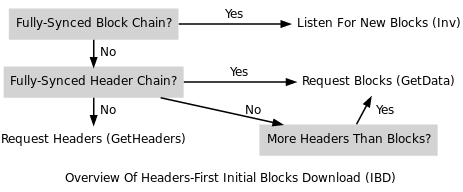
\includegraphics[width=9cm]{Image1.png}
	\centering		
	\caption{}
	\label{p5}
\end{figure}

La primera vez que se inicia un nodo tiene un bloque en su cadena de mejor bloque local: el bloque genesis codificado (bloque 0). El nodo elige un nodo remoto, que llamaremos nodo de sincronización, y le envía el mensaje ``getheader'':\\

\begin{figure}[h]
	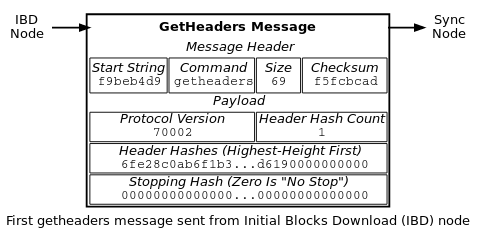
\includegraphics[width=10cm]{Image2.png}
	\centering		
	\caption{GetHeaders Message}
	\label{p5}
\end{figure}

En el campo de hash de cabecera del mensaje ``getheaders'', el nuevo nodo envía el hash de encabezado del único bloque que tiene, el bloque de generación (6fe2 ... 0000). También establece el campo de parada de hash en todos los ceros para solicitar una respuesta de tamaño máximo.\\

Una vez recibido el mensaje ``getheaders'', el nodo de sincronización toma el primer (y único) hash de encabezado y busca en su mejor cadena de bloque local un bloque con ese hash. Encuentra que el bloque 0 coincide, por lo que responde con un 2.000 cabeceras (respuesta máxima) a partir del bloque 1. Los hashes de estas cabeceras los manda en el mensaje mostrado a continuación:\\
\begin{figure}[h]
	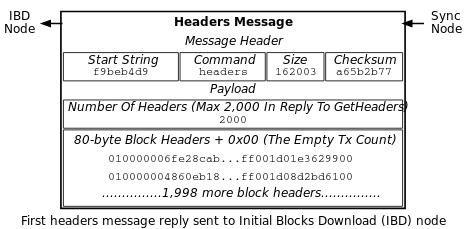
\includegraphics[width=10cm]{Image3.png}
	\centering		
	\caption{Headers Message}
	\label{p5}
\end{figure}

El nodo IBD puede validar parcialmente estos encabezados de bloque al garantizar que todos los campos sigan las reglas de consenso y que el hash del encabezado esté por debajo del umbral objetivo. (La validación completa requiere todas las transacciones del bloque).\\

Una vez validados parcialmente los encabezados se pueden hacer dos cosas en paralelo:

\begin{enumerate}
	\item \textbf{Descargar más encabezados:} el nodo IBD puede enviar otro ``getheader'' al nodo de sincronización para solicitar los próximos 2,000 encabezados. Esos encabezados pueden validarse inmediatamente y otro lote solicitarse repetidamente hasta que se reciba un mensaje desde el nodo de sincronización con menos de 2,000 encabezados, lo que indica que hemos acabado. Como resultado, la sincronización de cabeceras se puede completar en menos de 200 viajes redondos, aproximadamente 32 MB.\\

Una vez que el nodo IBD recibe un mensaje con menos de 2,000 encabezados, envía un mensaje de ``getheader'' a cada uno de sus peers salientes para obtener su vista de la mejor cadena de encabezado. Al comparar las respuestas, puede determinar fácilmente si los encabezados que ha descargado pertenecen a la mejor cadena de encabezado. Esto significa que un nodo de sincronización deshonesto se descubrirá incluso si no se utilizan los puntos de control.

	\item \textbf{Descargar bloques:} mientras el nodo IBD continúa descargando cabeceras, y después de que terminen de descargarse, el nodo IBD solicitará y descargará cada bloque. El nodo IBD puede usar los hash de las cabeceras de bloque que calculó desde la cadena de encabezado para crear mensajes ``getdata" que soliciten los bloques que necesita para su inventario. No necesita solicitarlos desde el nodo de sincronización; puede solicitarlos de cualquiera de los nodos completos a los que está conectado. Esto le permite buscar bloques en paralelo y evitar tener su velocidad de descarga restringida a la velocidad de carga de un solo nodo de sincronización.

Para distribuir la carga entre múltiples nodos, Bitcoin Core solo solicitará hasta 16 bloques a la vez desde un único nodo. Combinado con su máximo de 8 conexiones de salida, significa que la política ``Headers-First" solicitará un máximo de 128 bloques simultáneamente durante IBD.
\end{enumerate}

\subsection{Emisión de bloques}

Cuando un minero descubre un nuevo bloque, transmite el nuevo bloque a sus nodos conectados

\begin{itemize}

	\item \textbf{Unsolicited Block Push:} el minero envía un mensaje de bloque a cada uno de sus peers completos con el nuevo bloque.

	\item \textbf{Standard Block Relay:} el minero, que actúa como un nodo de retransmisor estándar, envía un mensaje \```inv'' a cada uno de sus nodos conectados con un inventario que hace referencia al nuevo bloque. Cada Header-First peer que quiere el bloque responde con un mensaje ``getheaders" seguido por ``getdata" que solicita el bloque completo. El minero responde en consecuencia a cada solicitud.

	\item \textbf{Direct Headers Announcement:} un nodo retransmisor puede omitir la sobrecarga de ida y vuelta de un mensaje \```inv'' seguido de encabezados obsoletos mediante el envio de un mensaje de encabezado que contiene el encabezado completo del nuevo bloque. Un par HF que recibe este mensaje seguirá el protocolo explicado. Un nodo HF puede indicar que prefiere recibir encabezados en lugar de \```inv'' enviando un mensaje especial ``sendheaders" durante el inicio de conexión. (Protocolo de la versión 0.12).

\end{itemize}

Por defecto, Bitcoin Core difunde bloques utilizando la política 3 a todos los nodos que han enviado señales con ``sendheaders'' y la 2 a los que no.

\subsubsection{Nodos huérfanos}

Bloques cuyo campo hash de encabezado del bloque anterior hace referencia a un encabezado de bloque que este nodo aún no ha visto, es decir, no tienen padres conocidos (a diferencia de los bloques obsoletos, que tienen padres conocidos pero que no forman parte de la mejor cadena de bloques).\\

Header-First evita parte de esta complejidad al solicitar siempre encabezados de bloque con el mensaje ``getheaders'' antes de solicitar un bloque con el mensaje ``getdata". El nodo emisor enviará un mensaje de encabezado que contiene todos los encabezados (hasta 2.000) que cree que el nodo de descarga necesita para alcanzar la punta de la mejor cadena de encabezado; cada uno de esos encabezados apuntará a su padre, por lo que cuando el nodo de descarga recibe el mensaje del bloque, no debe ser un bloque huérfano, se deben conocer todos sus padres (incluso si aún no se han validado). Si, a pesar de esto, el bloque recibido en el mensaje de bloque es un bloque huérfano, un primer nodo de encabezado lo descartará inmediatamente.

\begin{figure}[h]
	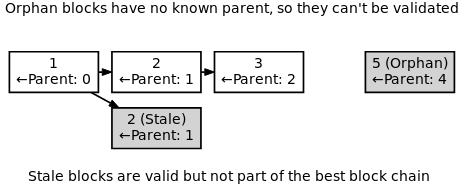
\includegraphics[width=10cm]{Image4.png}
	\centering		
	\caption{Bloques huérfanos}
	\label{p5}
\end{figure}

\subsection{Memory pool}

Los nodos completos pueden realizar un seguimiento de las transacciones no confirmadas que son elegibles para ser incluidas en el siguiente bloque. Esto es esencial para los mineros que realmente extraerán algunas o todas esas transacciones, pero también es útil para cualquier par que desee realizar un seguimiento de las transacciones no confirmadas.\\

Debido a que las transacciones no confirmadas no tienen un estado permanente en Bitcoin, se almacenan en memoria no persistente, llamándolas ``memory pool''. Cuando un par se apaga, su ``memory pool'' se pierde a excepción de cualquier transacción almacenada por su billetera ("wallet").\\

Las transacciones que se extraen en bloques que luego se vuelven obsoletos se pueden volver a agregar a ``memory pool''. Estas transacciones reagregadas se pueden volver a eliminar si los bloques de reemplazo las incluyen. Bitcoin Core elimina los bloques obsoletos de la cadena uno por uno, comenzando con la punta (bloque más alto).

\subsection{Nodos con mal comportamiento}

Existen mecanismos para castigar a los nodos que toman ancho de banda y recursos informáticos mediante el envío de información falsa. Si un peer obtiene un banscore por encima del umbral ($-banscore = <n>$), estará prohibido durante el número de segundos definidos por $-bantime = <n>$, que es 86400s=24h.

\section{Minado}

La minería agrega nuevos bloques a la cadena de bloques, por lo que es difícil modificar el historial de transacciones. Toma dos formas:

\subsection{Minería en solitario}

El minero intenta generar nuevos bloques por su cuenta, donde genera ganancias a partir del "premio" por bloque y de las tasas por transacción, siendo estas ganancias completas para dicho nodo.\\

Usan ``bitcoind" para obtener nuevas transacciones de la red. Su software de minería solicita periódicamente nuevas transacciones utilizando el RPC ``getblocktemplate", que proporciona la lista de nuevas transacciones más la clave pública a la que se debe enviar la transacción base. Recordemos que esta transacción unicamente puede ser generado por un nodo minero, que es la primera transacción de un nodo y que debe utilizar las ganancias de un nodo como entrada.\\

El software de minería construye un bloque usando una plantilla y crea un encabezado de bloque. A continuación, envía el encabezado del bloque de 80 bytes a su hardware de minería (un ASIC) junto con un umbral objetivo. El hardware de minería itera a través de cada valor posible para el encabezado del bloque y genera el hash correspondiente.\\

\begin{figure}[h]
	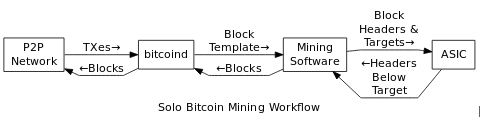
\includegraphics[width=11cm]{Image5.png}
	\centering		
	\caption{Minería}
	\label{p5}
\end{figure}

\subsection{Minería combinada}

El minero reúne recursos con otros mineros para encontrar bloques más a menudo, con los beneficios compartidos entre los mineros en una correlación aproximada con la cantidad de potencia de hashing que aportaron, permitiendo que el minero reciba pagos pequeños con una varianza menor.\\

El software de minería de cada minero se conecta al grupo y solicita la información que necesita para construir encabezados de bloque. El minero envía al grupo una copia de la información que el grupo necesita para validar que el encabezado tiene un hash debajo del objetivo y que el bloque de transacciones es válido para los propósitos del grupo.\\

La información que el minero envía al grupo se denomina participación porque demuestra que el minero hizo una parte del trabajo. Las tarifas de recompensa y transacción del bloque que provienen de la minería de ese bloque se pagan al grupo de minería. El grupo minero paga una parte de estos ingresos a mineros individuales en función de la cantidad de acciones que generan.

\begin{figure}[h]
	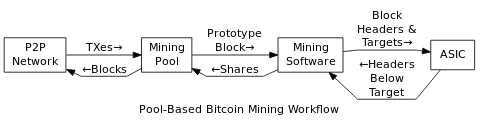
\includegraphics[width=11cm]{Image6.png}
	\centering		
	\caption{}
	\label{p5}
\end{figure}

\section{Bibliografía}
\begin{itemize}
	\item https://es.wikipedia.org/wiki/Peer-to-peer
	\item https://es.wikipedia.org/wiki/P2P\_privado
	\item https://es.wikipedia.org/wiki/Friend-to-friend
	\item https://es.wikipedia.org/wiki/Bitcoin
	\item https://en.wikipedia.org/wiki/Bitcoin\_network
	\item www.deic.uab.cat/~cperez/papers/FC2014-donet-perez-herrera.pdf
	\item https://bandaancha.eu/foros/todos-programas-p2p-aqui-839441
	\item https://es.wikipedia.org/wiki/Bitcoin
	\item https://en.wikipedia.org/wiki/Bitcoin
	\item https://www.bitcoin.com/
	\item https://en.bitcoin.it/wiki/
\end{itemize}

\end{document}